\section{New Graph--based Syntax}
The ultimate goal of the new graph--based syntax presented here is to be able to 
fully describe the fundamental problem formulation for a complex design task, 
while still being able to accomodate the more specific case when a solution 
strategy is applied to the problem formulation. In order to achieve that goal 
the graph needs to accomodate a number of constructs from MDAO problem: 

\begin{itemize}
    \item Analysis tools 
    \item Local and global variables 
    \item Information passing between analyses
    \item Coupling between analyses
    \item Design variables
    \item Objective or objectives 
    \item Local and global Constraints
    \item Iterative loops from solvers and optimizers
\end{itemize}

Beyond those basic constructs, there are also multiple three phases for a design process that 
all need to be representable with the new syntax. Firstly there is the initial problem definition
phase where the specific analysis tools and design goals are identified. At the end of this phase, 
a single formal problem formulation is selected specifying design variables, constraints, objectives, 
analysis tools, etc. Lastly some specifc procedure for solving the problem is selected, for example 
picking an MDAO optimization architecture. Using the proposed graph syntax, each of these phases 
can be represented with a related graph. 

\begin{itemize}
    \item Maximal Connectivity
    \item Fundamental Problem Formulation 
    \item Specific Solution Formulation
\end{itemize}

We present some transformations that can be applied to transition any graph
between any two adjacent design phases. The \emph{maximal connectivity graph} 
represents the full potential of all the analysis codes being considered, i.e. 
a large set of analysis codes being considered for a given problem are included in
a graph, with all possible connections between them also present. The second graph 
is \emph{fundamental problem formulation graph}, which is the smallest possible graph 
that still fully defines a given problem formulation. Finally, a \emph{specific problem formulation} 
may be represented by including additional edges and node types to represent the 
solution strategy being employed to solve the problem. 

The relationship between these three graphs is depicted in Figs.~\ref{f:tree} and \ref{f:hourglass}. 
The tree diagram demonstrates the fact that it is generally possible to obtain 
multiple FPFs from a single maximal connectivity graph. This  may correspond to 
different down--selections of analysis codes, different connections between them, 
or both. Each down--selection shrinks the number of possible FPFs that could be reached 
untill only one is remaining. Then, a single FPF, different SPFs may be obtained by implementing 
different solution strategies. The hourglass shape in Fig. \ref{f:hourglass} illustrates how 
the MCG gets reduced to a single FPF, then multiple possible SPFs exist to solve the problem.
In other words the FPF is obtained from the MCG by removing nodes and edges, 
and the SPF is obtained from the FPF by adding nodes and edges.

\begin{figure}[htb!]
    \centering
    \subfigure[number of possible graphs]{
    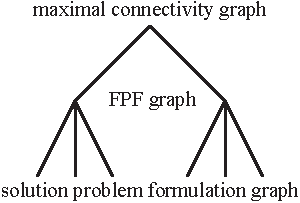
\includegraphics[width=2.0in]{images/tree}
    \label{f:tree}
    }
    \subfigure[graph size]{
    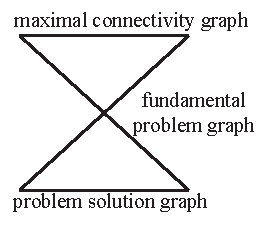
\includegraphics[width=2.0in]{images/hourglass}
    \label{f:hourglass}
    }
\caption{The relationship between the MCG, FPF, and SPF.}
\end{figure}

\subsection{Graph Theory Basics}
The notation used in this work is adapted from Diestel \cite{Diestel2010}. 
A \emph{graph} is a pair $G = (V,E)$ of sets such that $E \subseteq V \times V$, 
which means that the elements of $E$ are 2--element subsets of $V$. The set $V$ 
contains the \emph{vertices} or \emph{nodes} and the set $E$ contains the \emph{edges}.
For a \emph{directed graph*} we construct $E$ as a set of ordered pairs instead 
of a set of sets. Each ordered pair represents an edge starting at the node 
indicated by the first entry and directed to the node indicated by the second 
entry. Edge $e$ = $(x,y)$ may be referred to simply as $xy$ and we say $y = E(x)$. 

\begin{figure}[htb!]
	\begin{center}
	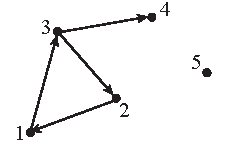
\includegraphics[width=1.5in]{images/example_directed_graph}
	\end{center}
	\vspace{-20pt}
\caption{Example directed graph.}
\label{f:example directed graph}
\end{figure}
As an example, for the directed graph shown in Fig.~\ref{f:example directed graph} we have
\begin{IEEEeqnarray*}{rCl}
V & = & \{1,2,3,4,5\}, \\
E & = & \big\{(1,2),(3,2),(1,3),(3,4)\big\}.
\end{IEEEeqnarray*}

Let $I$ be a nonempty set such that for each $i \in I$ there is a corresponding set $A_i$. The family $\{A_i | i \in I\}$ is an indexed family of sets with index $i$ and indexing set $I$, and we can say $\mathcal A = \{A_i | i \in I\}$\cite{smith2006}. Then the union over this family of sets is
\begin{equation}
\bigcup_{i \in I} A_i = \bigcup_{A \in \mathcal A} A = \{x | x \in A \txt{ for } A \in \mathcal A\}.
\end{equation}
Lastly, the cardinality of a set $B$ is the number of elements in $B$ and is denoted as $|B|$.

% \subsection{Problem Formulation Concepts to Represent}
% The MDAO problem formulation concepts we wish to represent are:
% \begin{description}
% \item[global input] A global input is a variable that is taken as given and is used by multiple analyses.
% \item[design variable]
% \item[function call] A function call requires a set of inputs to be fulfilled and has certain properties, such as run time, which are independent of the number of outputs actually being used.
% \item[passing of distinct variables] Instead of connecting analyses, the individual variables as are connected
% \item[objective \& constraint] These are variables that must be produced by the problem formulation for it to be valid
% \item[collision] A collision occurs when an input has multiple sources
% \item[hole] A hole occurs when an input has no sources
% \item[coupling] Couple is the mutual dependence between a set of analysis
% \item[multi--fidelity] It may be desirable for the same variable to be calculated by separate analyses and to use both results.
% \end{description}

\subsection{MDAO Graph Primatives}
There are three node types:  
\begin{description}
\item[variable node] represents passing of data.
\item[model node] represents the handling of data.
\item[driver node] represents constrol structures capable of managing iteration
\end{description}
There are two edge types: 
\begin{description}
\item[fixed edge] A fixed edge may never be removed from the graph.
\item[free edge] A free edge may be removed removed from the graph.
\end{description}

A number of restrictions are placed on the model node with respect to the number and 
type of edges that can be connected to it: 
\begin{enumerate}
\item A model node can only have one edge directed to or from another model node.
\item A model node can only have fixed edges directed in or out.
\item A model node must have at least one edge directed in and at least one edge directed out.
\item If a variable node with an outgoing edge to a model node may not have any other outgoing edges.
\end{enumerate}

Analysis tools take in a number input variables, then perform some work to calculate 
the values for their respective outputs. In an MDAO graph, this process is 
represented by an group of nodes and edges called an \emph{analysis block}, 
shown in Fig. \ref{f:analysis block}. Within an analysis block each variable 
node represents a single input or output and is connected 
to a single model node via a fixed edge. Note that in Fig. \ref{f:analysis block}, 
the analysis block contains two model nodes, with a single edge connecting them. 
This part of the graph represents the necessary calculations to map given inputs 
to proper output values. Although analysis blocks are comprised of multiple nodes and edges, since all 
the edges within them are fixed, they become fixed structures within a graph.

\begin{figure}[htb!]
    \begin{center}
    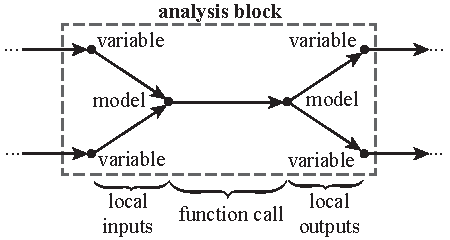
\includegraphics[width=4in]{images/analysis_block}
    \end{center}
    \vspace{-10pt}
\caption{Example analysis block. The each node type and edge type is labeled in italics and annotated parenthetically.}
\label{f:analysis block}
\end{figure}

Via the analysis block structure, we can also distinguish between input and ouptut
variable nodes. Inputs are any variable nodes that have an outgoing edge into a model 
node. Conversely, outputs are any variable nodes that have an incoming edge from a model node. 
Note that by this definition, inputs and outputs can only exist when variable nodes poses an 
edge joining them to a model node. In Fig. \ref{f:analysis block} these are labeled out as 
local inputs and local outputs. The necessity to be connected to a specific model node forces
the variable nodes to be local in nature. When information from the output of one analysis 
block is passed, or connected, to the input of another analysis block, a new free edge is added 
connecting the two variable nodes involved in the exchange. The edge is free because, unlike the edges 
within an analysis block, it could be added or removed depending on the demands of the specific problem. 

The MDO problem formulation concepts represented by nodes are given in 
Table \ref{t:node representation}, and the concepts represented by edges are 
given in Table \ref{t:edge representation}.
% \begin{itemize}
% \item An objective or constraint is indicated by a variable node with no outgoing edges and with the incoming edges being directed from only other variable nodes.
% \item A global input is a variable node with no edges directed in and with at least two edges directed out to different variable nodes.
% \item A design variable is represented by a variable node with no edges directed in and on fixed edge directed out.
% \end{itemize}
\begin{table}[h!]
 \begin{center}
  \caption{Problem formulation concept represented by a node}
  \label{t:node representation}
  \begin{tabular}{ccc} \hline 
edges directed in & edges directed out & node representation \\ \hline
only free edges & none & objective or constraint\\
none & at least two free edges & global input \\
none & one fixed edge & design variable \\ \hline
  \end{tabular}
 \end{center}
 \vspace{-15pt}
\end{table}
\begin{table}[h!]
 \begin{center}
  \caption{Problem formulation concept represented by an edge}
  \label{t:edge representation}
  \begin{tabular}{ccc} \hline 
from node & to node & edge representation \\ \hline
variable & variable & connection/passing of a variable\\
variable & model & local input \\
model & variable & local output \\
model & model & function call \\ \hline
  \end{tabular}
 \end{center}
 \vspace{-15pt}
\end{table}
%`Connection' edges connect the local outputs from one analysis block to input nodes.

\section{Graph--based Representation of the Fundamental Problem Formulation}


In this section we introduce the remaining necessary notion and give graph--theory based definitions of the MCG and FPF, and then process to demonstrate how the FPF is obtained from the MCG.

\subsection{Additional Notation}
For node $v \in V$ the edges directed out are given by $E(v)$ and the edges directed into $v$ are given by $E^{-1}(v)$; $E(E(v))$ is denoted as $E^2(v)$, and likewise for additional levels. 
The \emph{indegree} of a node is the number of edges directed in and is denoted as $\txt{deg}^-(v)$, and the \emph{outdegree} is the number of edges directed out and it is denoted as $\txt{deg}^+(v)$.
We also define the \emph{upper indegree limit} 
\begin{equation}
\txt{deg}_u^-(v):V \to \mathbb{N}
\end{equation} 
and the \emph{lower indegree limit}
\begin{equation}
\txt{deg}_l^-(v):V \to \mathbb{N}.
\end{equation}
These user-specified limits set the number of edges that may be directed into a node for a problem formulation to be valid. For example, a variable node $v$ will have $\txt{deg}_u^-(v) = \txt{deg}_l^-(v) = 1$, unless it is a multi--fidelity variable, in which case the user may specify some upper limit higher than one.

To keep track of which nodes and edges are which type, let $T_\txt{node}$ and $T_\txt{edge}$ be sets containing the possible node types and edge types, respectively, and then define mappings $t_\txt{node}:V \to T_\txt{node}$ and $t_\txt{edge}:E \to T_\txt{edge}$ to assign a type to each node and edge.
Then, for example, for a variable node $v$ we have $t_\txt{node}(v) = \txt{`variable'}$.


 % A \emph{path} is a nonempty graph $P = (V,E)$ with $V = \{x_0,x_1,\ldots,x_k\}$ and $E = \{x_0x_1,x_1x_2,\ldots,x_{k-1}x_k\}$, where $x_i$ are all distinct. A graph $G$ is \emph{connected} if any two of its vertices are linked by a path in $G$. A \emph{tree} is a connected and acyclic graph.
%%% this needs to be changed to fit the definition using a directed graph


\subsection{Maximal Connectivity Graph}
To construct the maximal connectivity graph, we assume that a set of codes, global inputs, and objectives and constraints (collectively called global outputs). The codes are represented by analysis blocks $A_i=(V_{A_i},E_{A_i}), \ i\in \{1,2,\ldots,m\}=I$, the global inputs are represented a set of variable nodes $V_\txt{in}$, and the global outputs are represented by a set of variable nodes $V_\txt{out}$. We assume that $V_\txt{in}$, $V_\txt{out}$, and $A_i$ are given, and that any potential connection between variables is given in the form of the free edges in the set $C_M$. 
Then we may construct the maximal connectivity graph $M=(V_M,E_M)$ as
\begin{IEEEeqnarray*}{rCl}
V_M & = & V_\txt{in} \cup V_\txt{out} \cup \left( \bigcup_{i \in I} V_{A_i} \right), \\
E_M & = & C_M \cup \left( \bigcup_{i \in I} E_{A_i} \right),
\end{IEEEeqnarray*}
The MCG $M$ is uniquely determined by the given set of analysis blocks, the required outputs, and the given global inputs. In the cases where the set of global inputs $I$ is not known a priori, the process of obtaining the FPF will reveal the required inputs, as discussed subsequently.

\subsection{Fundamental Problem Formulation Graph}
We now define the fundamental problem formulation graph, $F=(V_F,E_F)$, as a directed graph meeting the following conditions
\begin{enumerate}
\item[(1)] $\displaystyle{I_F \subset I}$ such that the following conditions hold
\item[(2)] $\displaystyle{ \forall i \in I, \ \exists v \in V_{A_i} \txt{ with } t_\txt{node}(E^{-1}(v))=\txt{`model'} \txt{ and } \txt{deg}^+(v)>0 }$
%\item[(3)] $\displaystyle{ \forall i \in I, \forall v \in V_{A_i} \txt{ with } t_\txt{node}(v) = \txt{`variable,'} \  \txt{deg}_l^-(v) < \txt{deg}^-(v) \leq \txt{deg}_u^-(v)}$
%\item[(3)] $\displaystyle{ \forall i \in I, \forall v \in V_\txt{out} \txt{ with } t_\txt{node}(v) = \txt{`variable,'} \  \txt{deg}_l^-(v) < \txt{deg}^-(v) \leq \txt{deg}_u^-(v)}$
\item[(3)] $\displaystyle{V_{\txt{in},F} = \{v \in V_\txt{in} | \txt{deg}^+(v) > 0\} }$
\item[(4)] $\displaystyle{V_F = V_{\txt{in},F} \cup V_\txt{out} \cup \left( \bigcup_{i \in I_F} V_{A_i} \right)}$
\item[(5)] $\displaystyle{E_F = C_F \cup \left( \bigcup_{i \in I_F} E_{A_i} \right), \ C_F \subset C_M}$
\item[(6)] $\displaystyle{\forall v \in V_F \txt{ with } t_\txt{node}(v) = \txt{`variable,'} \  \txt{deg}_l^-(v) \leq \txt{deg}^-(v) \leq \txt{deg}_u^-(v)}$
\end{enumerate}
The set $I_F$ is an index set containing the indices of the analysis blocks in $F$ and it may only include the analysis blocks $A_i$ that meet requirements (2) and (6). Requirement (2) stipulates that the analysis blocks in $F$ must each have at least one local output that is beging used. Requirement (3) stipulates that only the global inputs that are being used should be included. Lastly, requirement (6) stipulates that the number of edges directed into the variable nodes must be within the lower and upper indegree limits; if $\txt{deg}^-(v) < \txt{deg}_l^-(v)$ the node is called a \emph{hole}, and if $\txt{deg}^-(v) > \txt{deg}_u^-(v)$ the node is called a \emph{collision}. 

The set $C_F$ is a set containing free edges representing connections. Since $C_M$ is the set of all potential connections, we must have $C_F \subset C_M$. While no other conditions are explicitly stated for $C_F$, requirement (6) is actually a requirement on both $I$ and $C_F$.

\subsection{Obtaining the Fundamental Problem Formulation Graph}
In general, there may be multiple different graphs that satisfy the FPF conditions, though there may be none at all. Here, we describe a process for obtaining an FPF by starting with the MCG and disconnecting free edges until the FPF conditions are met. Then the problem is reduced to deciding which free edges to remove.

%Then, mathematically, the FPF starts with $\mathcal A_1 = \{1,\ldots,m\}$, $I_{F,1} = I$, and $C_{F,1} = C_M$.
Then, mathematically, the FPF starts with $C_{F,0} = C_M$.
First address the nodes where $\txt{deg}^-(v) < \txt{deg}_l^-(v)$ then the ones where $\txt{deg}^-(v) > \txt{deg}_u^-(v)$

\begin{enumerate}
\item The first step is to detect holes and disconnect the free edges following them. These free edges are removed because they represent variables which cannot be determined because the analysis function does not have adequate inputs. The set of variable nodes which are holes is created as
\begin{equation}
H = \{v \in V | t_\txt{node}(v) = \txt{`variable'} \txt{ and } \txt{deg}^-(v) < \txt{deg}_l^-(v) \},
\end{equation}
which is the set of variable nodes with few incoming edges than are allowed by the lower indegree limit.
Then the updated set of edges is created by removing the first set of free edges following the hole:
\begin{equation}
C_{F,1} = C_{F,0} \setminus \{(x,y) \in E | x=E^3(v) \txt{ for } v \in H\},
\end{equation}
%deg-v is now recaculated for the new C. 
and this step is demonstrated by Fig.~\ref{f:holes}. Because removing these edges can create new holes, this step must be repeated until no more holes are found.
\begin{figure}[htb!]
	\begin{center}
	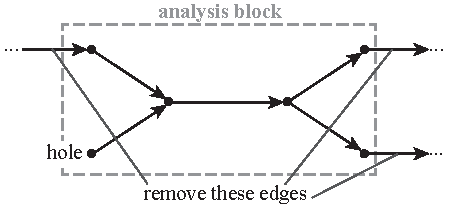
\includegraphics[width=3in]{images/analysis_block_hole}
	\end{center}
	\vspace{-20pt}
\caption{Example variable node indicating a hole.}
\label{f:holes}
\end{figure}
\item The second step is to detect collisions and to then disconnect enough free edges so that the collisions are resolved. The set of variable nodes which contain collisions is created as
\begin{equation}
S_\txt{nodes} = \{v \in V | t_\txt{node}(v) = \txt{`variable'} \txt{ and } \txt{deg}^-(v) > \txt{deg}_u^-(v) \}.
\end{equation}
For each collision node we can construct a set contained the edges directed in. The set containing all of these sets is constructed as
\begin{equation}
S_\txt{edges} = \big \{ \{(x,y) \in E\} \big | y \in S_\txt{nodes} \big \}
\end{equation}
Let $J=\{1,2,\ldots,|S_\txt{edges}|\}$ be an indexing set for $S_\txt{edges}$ such that each $S_{\txt{edges},j}$ corresponds to a set in $S_\txt{edges}$ for $j \in J$. We can assume that $J$ also indexes $S_\txt{nodes}$ because there is a one--to--one correspondence between the elements in $S_\txt{nodes}$ and the elements in $S_\txt{edges}$. Then we may construct sets of edges as
\begin{equation}
B_j = \big \{e_k \in S_{\txt{edges},j} \ | \ k \in \{1,2,\ldots,K\} \txt{ with } K \leq \txt{deg}_u^-(v_j) \big \}, \ j \in J,
\end{equation}
which means that each set $B_j$ is constructed from the set $S_{\txt{edges},j}$ by taking only as many edges as are allowed by the upper indegree limit of $v_j$. The construction of each $B_j$ corresponds to making a decision on which edges to include and which edges not to include. Then let
\begin{equation}
C_{F,2} = \{ e \in C_{F,1} \ | \ e \in B_j \txt{ for some } j \in J\}.
\end{equation}
\item The third and final step is to remove any unused nodes and edges. The set of unused variable nodes representing local outputs is
\begin{equation}
V_\txt{empty} = \{v \in V_M \ | \ t_\txt{node}(E^{-1}(v))=\txt{`model'} \txt{ and } \txt{deg}^+(v) = 0\},
\end{equation}
and so then the indexing set for only the analysis blocks with at least one used local output may be constructed as
\begin{equation}
I_3 =  \{i \in I \ | \ \nexists v \in V_{A_i} \txt{ such that }  v \in V_\txt{empty} \}.
\end{equation}
Finally, the set of nodes and edges describing a fundamental problem formulation is given by
\begin{equation}
V_{F,3} = V_M \setminus V_\txt{empty}
\end{equation}
\begin{equation}
C_{F,3} = \{ (x,y) \in C_{F,2} \ | \ x \in V_{A_i} \txt{ or } y \in V_{A_i} \txt{ for some } i \in I_3 \}
\end{equation}
\begin{equation}
F_3 = (V_{F,3},C_{F,3})
\end{equation}


%Let $F_2 = (V_M,C_{F,2})$ be an undirected graph, which is to say to disregard the directions associated with $C_{F,2}$. 


%Fixed edges are fixed only with respect to the analysis block in which they reside, it is okay to remove them along with the entire analysis block.

\end{enumerate}



    \subsection{Solution Graph Syntax}
    What is the difference between a problem formulation and a problem solution method? Convert from a cyclic graph, to an acyclic graph
    \begin{itemize}
        \item Cycles indicate convergence loops or design variable loops
        \item Problem can't be solved until all loops are *removed* by adding solvers/optimizers
        \item *Special* nodes for solvers and optimizers that *break* loops (from an algorithmic point of view)
        \item FPF represents the minimal amount of information necessary to define a problem
        \item Any solution path grows the graph complexity by adding edges and nodes (or possibly have an empty solution graph, which you build up
        as you remove edges from problem formulation graph?)
    \end{itemize}
